A manufatura aditiva é o processo de fabricação a partir de adição de camadas de materiais com base em dados de
CAD-3D \cite{manufatura_aditiva}. Manufatura aditiva é o nome que se dá para impressão 3D, se constituindo como
terceiro pilar na tecnologia de manufatura, que inclui também a "manufatura subtrativa" (mais conhecido como processos
de usinagem) e a "manufatura formativa" (como fundição, injeção e conformação).

Como ilustrado na figura \ref{fig:manufatura_aditiva}, asas etapas típicas da manufatura aditiva são:

\begin{enumerate}
	\item Obtenção do modelo CAD 3D;
	\item Fatiamento do modelo e obtenção o contorno das camadas;
	\item Adição de camadas de materiais;
	\item Obtenção do produto final.
\end{enumerate}

O modelo é fatiado por meio de um software, e o resultado é geralmente um conjunto de contornos de mesma espessura.
Esse conjunto de contornos é convertido em comandos a serem executados por uma máquina, em ações de processamento das
camadas. No caso de uma impressora 3D de filamento, o software que obtém as informações de camadas converte essas
informações em código G, linguagem padronizada para máquinas CNC.

\begin{figure}[h]
	\centering
	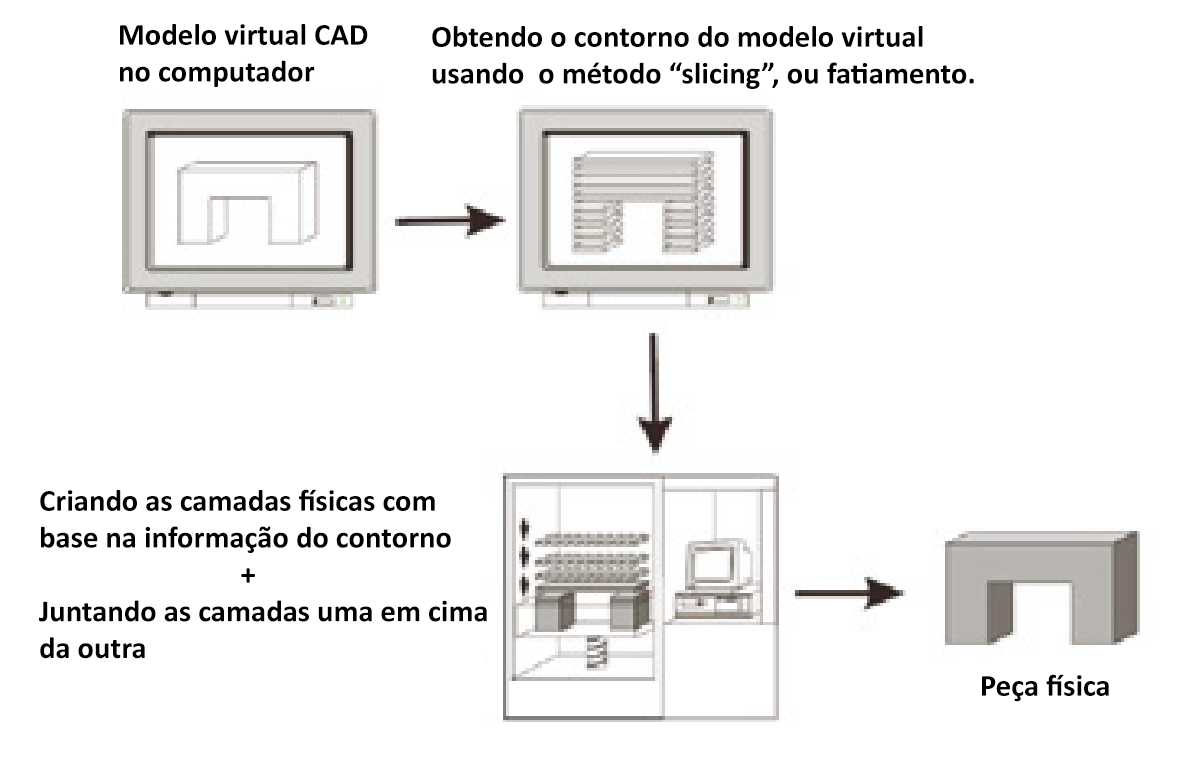
\includegraphics[width=1\textwidth]{figures/manufatura_aditiva}
	\caption{Processo de manufatura aditiva \cite{manufatura_aditiva}}
	\label{fig:manufatura_aditiva}
\end{figure}
